%%%%%%%%%%%%%%%%%%%%%%%%%%%%%%%%%%%%%%%%%%%%%%%%%%%%%%%%
%%%%%%%%%%%%%%%%%%%%%%%%%%%%%%%%%%%%%%%%%%%%%%%%%%%%%%%%
\section[Theory]{The Standard Model and beyond}
\setcounter{tocdepth}{2}

\begin{frame}
\tikz[remember picture,overlay]{\node (b) at (0.42\paperwidth,-0.1\paperheight) [inner sep=0pt,opacity=0.4]{
\includegraphics[width=1.0\paperwidth]{FeynBongo.jpg}};}
\begin{center}
The Standard Model and beyond
\end{center}
\end{frame}

\subsection{Theory}
\begin{frame}{The Standard Model}
\vspace{-.2cm}
\begin{columns}

\begin{column}{.50\textwidth}
\begin{block}{}
\begin{itemize}\scriptsize
%\item Theory developed from quantum theory and special relativity -> Quantum Field Theory (Feynman, Dirac, ...) + Continuous group symmetries (Noether, Yang, ...)
\item Model developed from quantum theory and special relativity $\to$ Quantum Field Theory + Continuous group symmetries
\item Fermions: matter components (electron, muon, quarks...)
\item Bosons: interaction mediators (\W, \Z, ...)
\item Extremely successful model: \\ quarks, CKM, \W~and \Z~masses, ...
\item But it is limited:
  \begin{itemize}\scriptsize
  \item Neutrino masses
  \item Dark matter
  \item \textbf{Hierarchy problem}
  \end{itemize}
\end{itemize}
\end{block}
\end{column}

\begin{column}{.50\textwidth}
\begin{figure}[!Hhtbp]
  \begin{center}
    \includegraphics[width=1.0\textwidth]{Standard_Model_of_Elementary_Particles.jpg}\\
    \vspace{.6cm}
    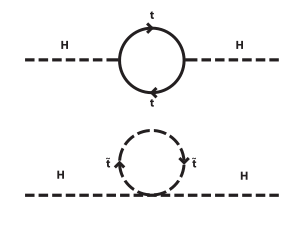
\includegraphics[width=0.8\textwidth]{SUSY.png}
    %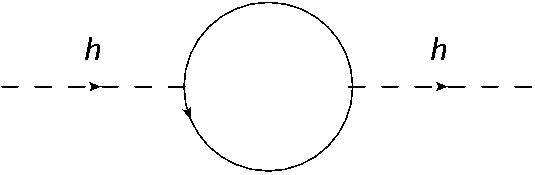
\includegraphics[width=0.8\textwidth]{../figs/HierarchyLoop.png}
    %\caption{Particle content of the standard model.}
    %\label{fig:SMContent}
  \end{center}
\end{figure}
\end{column}
\end{columns}
\end{frame}


\begin{frame}{Vector Like Quarks (VLQ)}
\vspace{-.3cm}
\begin{columns}

\begin{column}{.40\textwidth}
\begin{block}{}
\begin{itemize}\scriptsize
\item Motivated by the hierarchy problem $\to$ New states to cancel loop contributions
\item SM + not chiral quarks
\item States:
  \begin{itemize}\scriptsize
  \item $X$ 5/3 e
  \item \textbf{\Tp~2/3 e (as the top)}
  \item $B$ -1/3 e (as the b)
  \item $Y$ -4/3 e
  \end{itemize}
%\item \textbf{Generically they can be mixed with the three SM-quark generations}
%\item Produced in pairs or in single production mode with a SM-quark
%\item $T'\to bW^{+/-}, tZ^{0}, tH^{0}$
\end{itemize}
\end{block}
\end{column}

\begin{column}{.60\textwidth}
%\begin{figure}[!Hhtbp]
%  \begin{center}
%    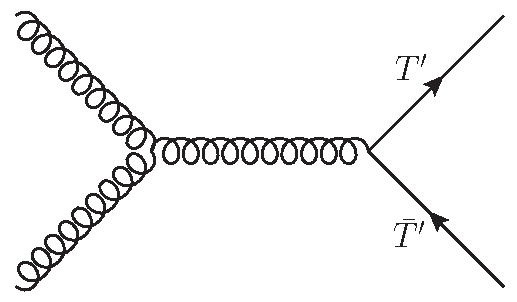
\includegraphics[width=0.5\textwidth]{../figs/Gluon_fusion_T_pair.jpg}
%    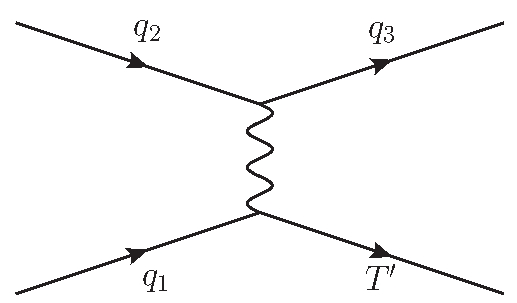
\includegraphics[width=0.5\textwidth]{../figs/Tchannel_T_single.jpg}
%  \end{center}
%\end{figure}
\tiny{
\begin{eqnarray}
  \mathcal{L}_{\binom{X}{T'}} & = & \kappa_{T}\left\{ \sqrt{\frac{\zeta_{i}\xi_{Z}^{T}}{\Gamma_{Z}^{0}}}\frac{g}{2c_{W}}\left[ \bar{T'}_{R}Z_{\mu}\gamma^{\mu}u^{i}_{R}\right]\right\} \nonumber\\
              & - & \kappa_{T}\left\{ \sqrt{\frac{\zeta_{i}\xi_{H}^{T}}{\Gamma_{H}^{0}}}\frac{M}{v}\left[ \bar{T'}_{L}Hu^{i}_{R}\right] + \sqrt{\frac{\zeta_{3}\xi_{H}^{T}}{\Gamma_{H}^{0}}}\frac{m_{t}}{v}\left[ \bar{T'}_{R}Ht_{L}\right]\right\} \nonumber\\            
              & + & \kappa_{X}\left\{ \sqrt{\frac{\zeta_{i}}{\Gamma_{W}^{0}}}\frac{g}{\sqrt{2}}\left[ \bar{X}_{R}W^{+}_{\mu}\gamma^{\mu}u^{i}_{R}\right]\right\} +h.c. \nonumber
\end{eqnarray}
}%
\vspace{-.2cm}
\begin{block}{}
\begin{itemize}\scriptsize
\item $\xi_{Z}^{T},\xi_{H}^{T}$ coupling to \Z~and \Hb, fixed by representation. 
\item $\zeta_{i}$ coupling to SM quarks.
\item In general: $T'\to bW^{+/-}, tZ^{0}, tH^{0}$
\end{itemize}
\end{block}

\end{column}
\end{columns}

\vspace{-.2cm}
\begin{center}
\resizebox{\textwidth}{!}{
\begin{tabular}{|c|c|c|c|c|c|c|c|c|}
\hline 
 & SM & \multicolumn{2}{c|}{Singlets} & \multicolumn{3}{c|}{Doublets}  & \multicolumn{2}{c|}{Triplets} \\
 & $\binom{u}{d}$ $\binom{c}{s}$ $\binom{b}{t}$ & \Tp & $B$ & $\binom{X}{T'}$ & $\binom{T'}{B}$ & $\binom{B}{Y}$ & $\left(\begin{array}{c} X \\ T' \\ B \end{array} \right)$ & $\left(\begin{array}{c} T' \\ B \\ Y \end{array} \right)$ \\ 
\hline
$SU(2)_{L}$ & 2 & \multicolumn{2}{c|}{1} & \multicolumn{3}{c|}{2} & \multicolumn{2}{c|}{3} \\ \hline
$U(1)_{Y}$ & $q_{L}=1/6$; $u_{R}=2/3$; $d_{R}=-1/3$ & 2/3 & -1/3 & 7/6 & 1/6 & -5/6 & 2/3 & -1/3 \\
\hline
\end{tabular}
}
%\caption{Possible VLQ representations and corresponding $SU(2)_{L}\times U(1)$ charges and SM quarks. \label{tab:VLQRepre}}
\end{center}

%\begin{figure}[!Hhtbp]
%  \begin{center}
%    \includegraphics[width=0.4\textwidth]{../figs/pheno_prod_single_tp.png}
%    \includegraphics[width=0.4\textwidth]{../figs/pheno_prod_pair_tp.png}
%  \end{center}
%\end{figure}

\end{frame}


\begin{frame}{Non-standard doublet $\binom{X}{T'}$}
\vspace{-.3cm}

\begin{block}{}
\begin{itemize}\scriptsize
\item \Tp~couplings to light quarks maximized
\item $M(T')\in [600,1000]$ \GeVcc, 8 TeV considered
\item $\sigma_{pp\to T'j} > \sigma_{pp\to T'T'}$
\item $Br(T' \to tH^{0})=0.5$
\end{itemize}
\end{block}

\vspace{.3cm}
\begin{figure}[!Hhtbp]
  \begin{center}
    \includegraphics[width=0.5\textwidth]{pheno_prod_single_tp.png}
    \includegraphics[width=0.5\textwidth]{pheno_prod_pair_tp.png}
  \end{center}
\end{figure}

\end{frame}


\begin{frame}{Signal topology}
\vspace{-.2cm}
\begin{center}
    \includegraphics[width=1.0\textwidth]{Tprime_scheme.png}
  \end{center}
\end{frame}



\begin{frame}{Current limits}
\vspace{-.2cm}
%\begin{center}
\includegraphics[width=0.75\textwidth]{../figs/Ana/ATLAS_VLQ_TT_step4.png}\\
\begin{center}
\includegraphics[width=0.4\textwidth]{../figs/Ana/CMS-B2G-13-005_Figure_010-a.png}
\includegraphics[width=0.4\textwidth]{../figs/Ana/CMS-B2G-13-005_Figure_010-b.png}
  \end{center}
\begin{textblock}{25}(95,30)\scriptsize
Searches mainly looking for pair production and leptonic channels 
\end{textblock}

\end{frame}







\iffalse
\begin{frame}{}
\vspace{-.2cm}
\begin{center}
    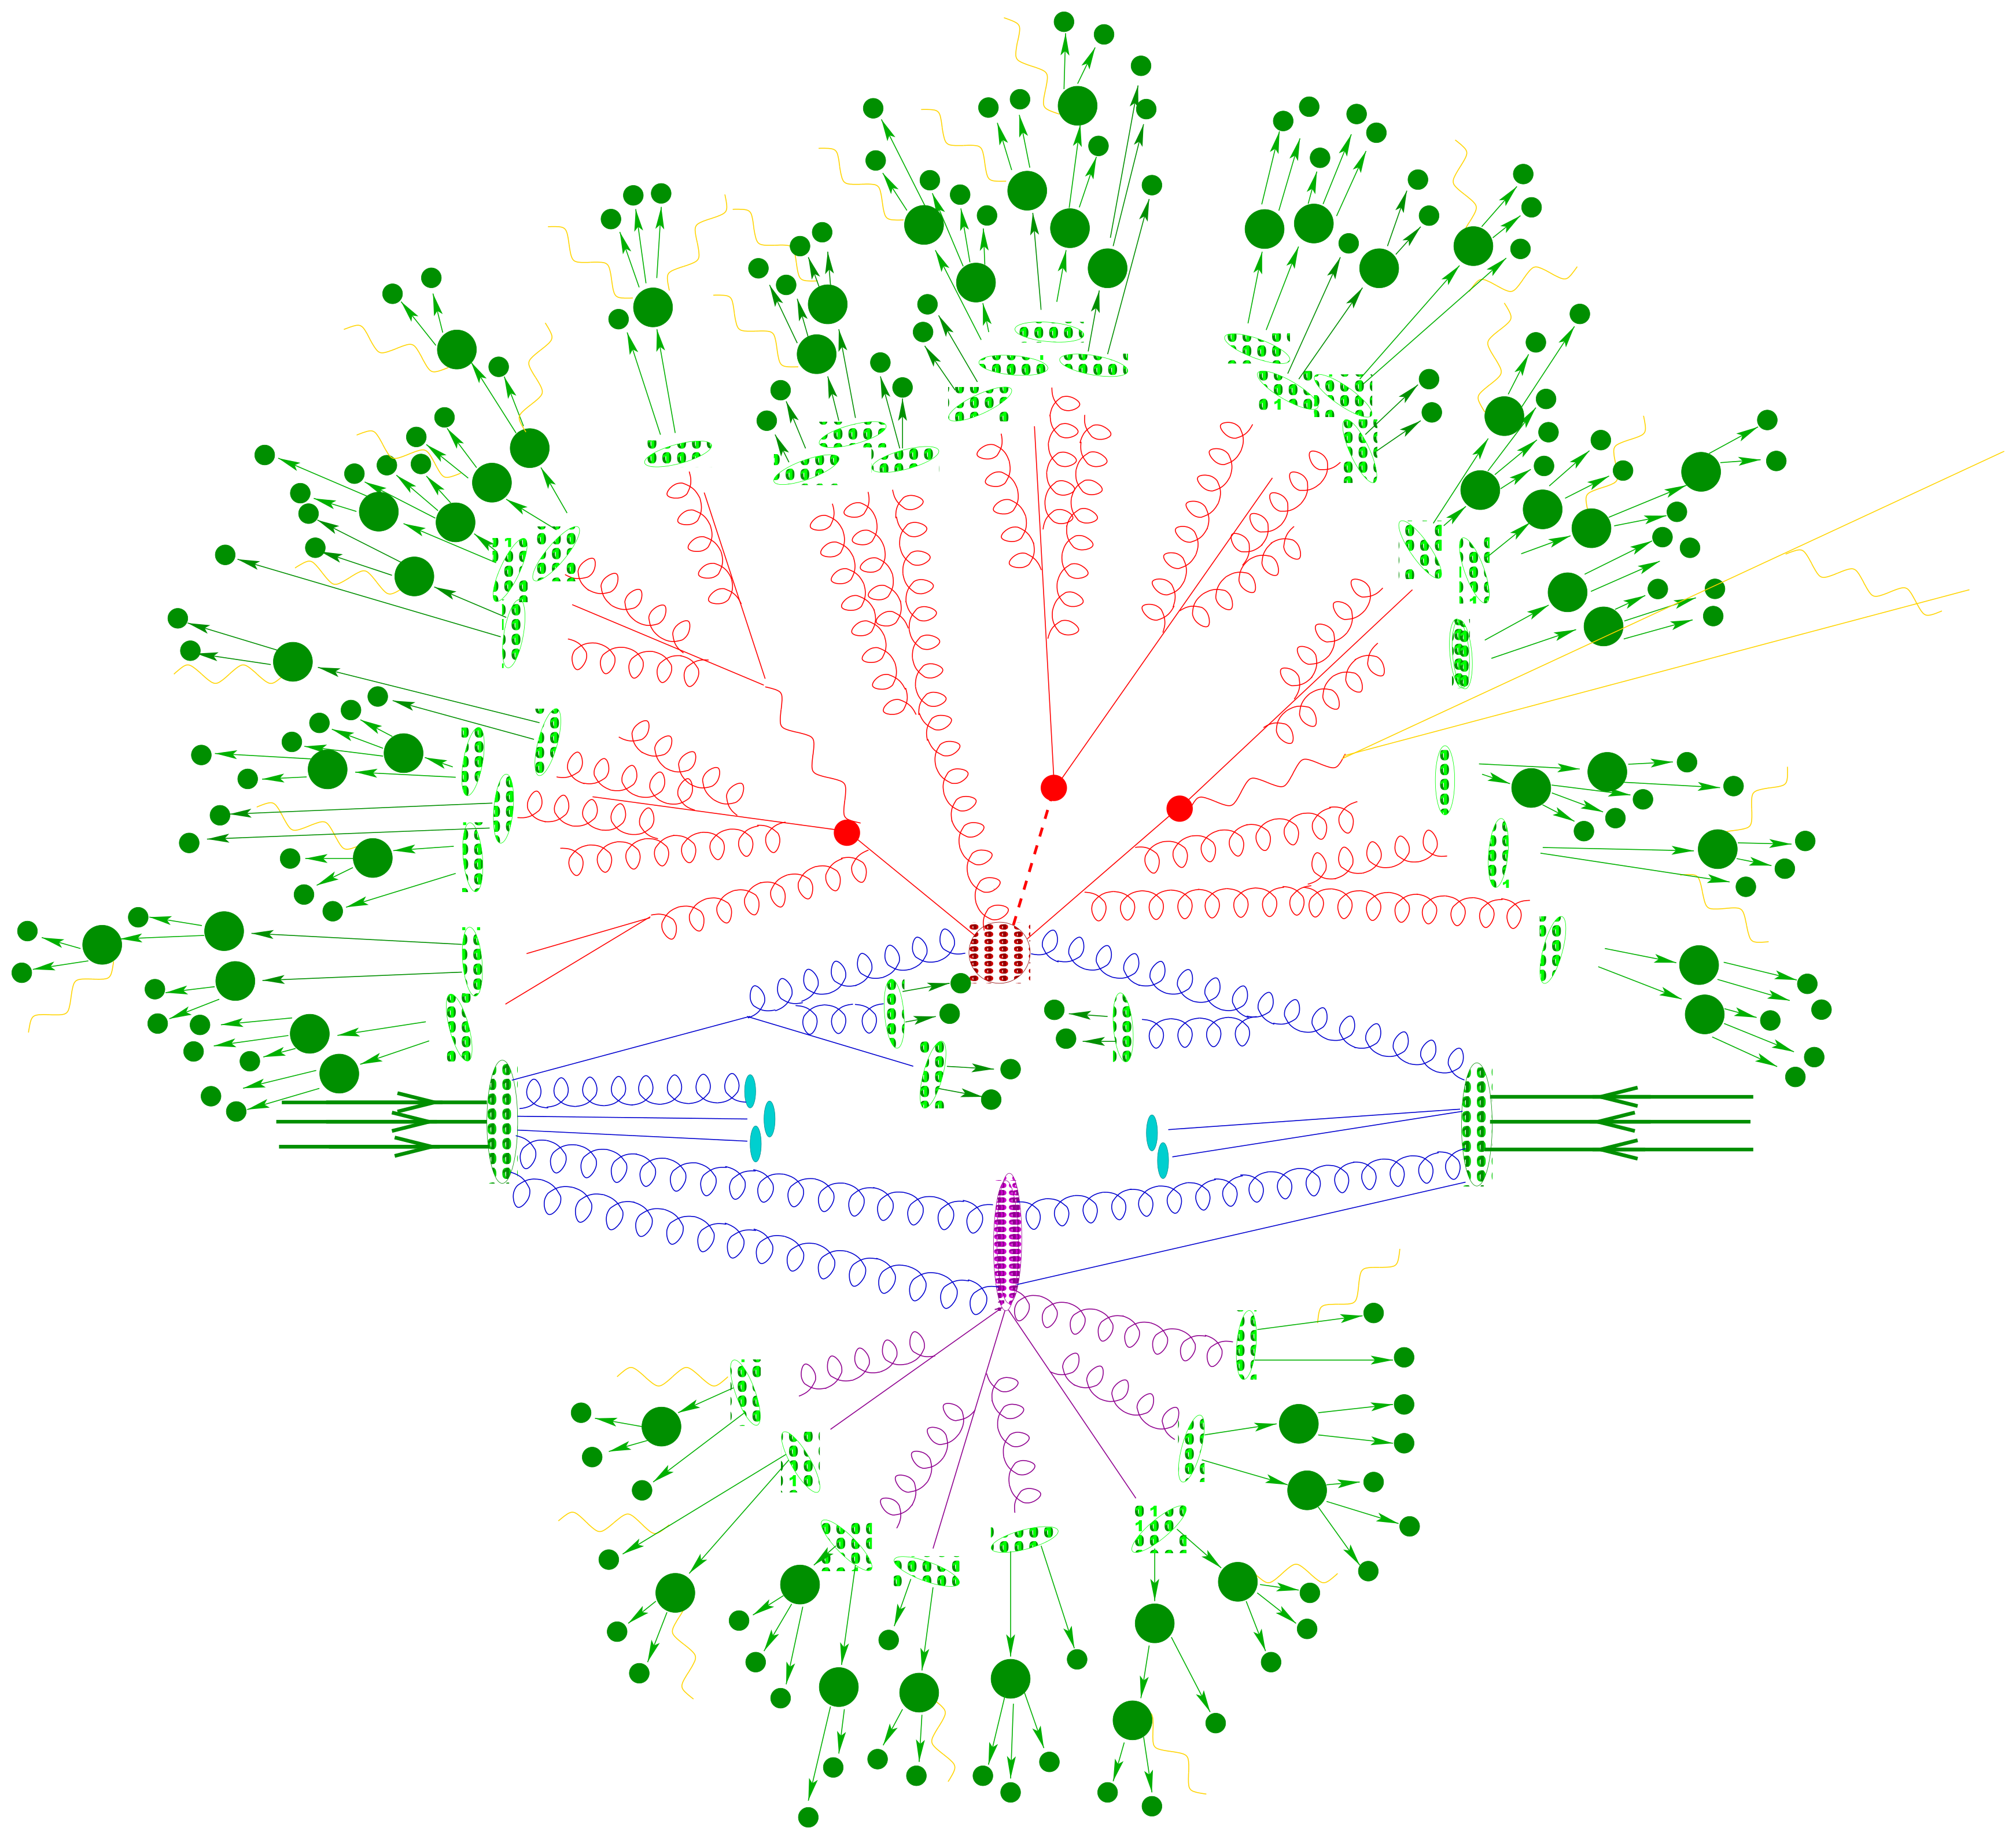
\includegraphics[width=0.9\textwidth]{parton_shower.png}
  \end{center}
\end{frame}


\begin{frame}{SM at the LHC}
\vspace{-.3cm}
\begin{columns}

\begin{column}{.50\textwidth}
\begin{block}{Top quark production}
\begin{itemize}\tiny
\item Heaviest quark in the SM 
\item LHC as a top machine $\to$ 6 tops/s (5 from pair, 1 from single)
\item 8 TeV: $\sigma_{t\bar{t}}=247.47\pm12.37$ pb, $\sigma_{t,\; \text{s-channel}}=5.56\pm0.22$ pb, $\sigma_{t,\; \text{t-channel}}=84.34\pm1.69$ pb and $\sigma_{tW}=22.2\pm0.67$ pb
\item $t\to bW^{-}$ with $Br(W^{+/-}\to l\nu)=0.33$ and $Br(W^{+/-}\to q\bar{q}')=0.67$
\item $m_{t}=173.34\pm 0.76$ \GeVcc
\end{itemize}
\end{block}

\vspace{-.4cm}
\begin{figure}[!Hhtbp]
  \begin{center}
    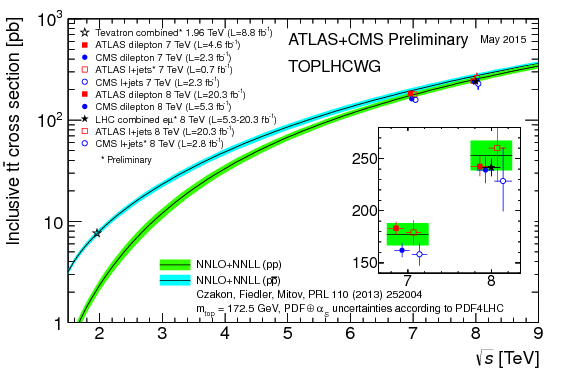
\includegraphics[width=1.0\textwidth]{../figs/toplhcwg_ttxsec_sqrts_may2015.png}
    %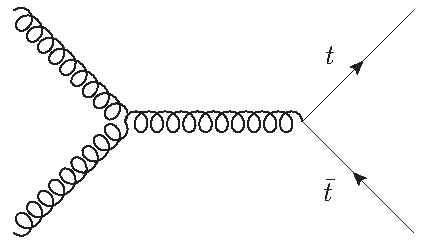
\includegraphics[width=0.3\textwidth]{../figs/Gluon_fusion_top_pair.jpg}
  \end{center}
\end{figure}
\end{column}

\begin{column}{.50\textwidth}
\begin{block}{Higgs boson production}
\begin{itemize}\tiny
\item Heaviest boson in the SM 
\item Rare process: 20 pb at 8TeV
\item Many decay channels: $Br(H^{o}\to b\bar{b})=0.57$
\item $m_{H}=125.09\pm 0.24$ \GeVcc~and $\sigma_{H}<20$ MeV
\end{itemize}
\end{block}

\vspace{-.2cm}
\begin{figure}[!Hhtbp]
  \begin{center}
    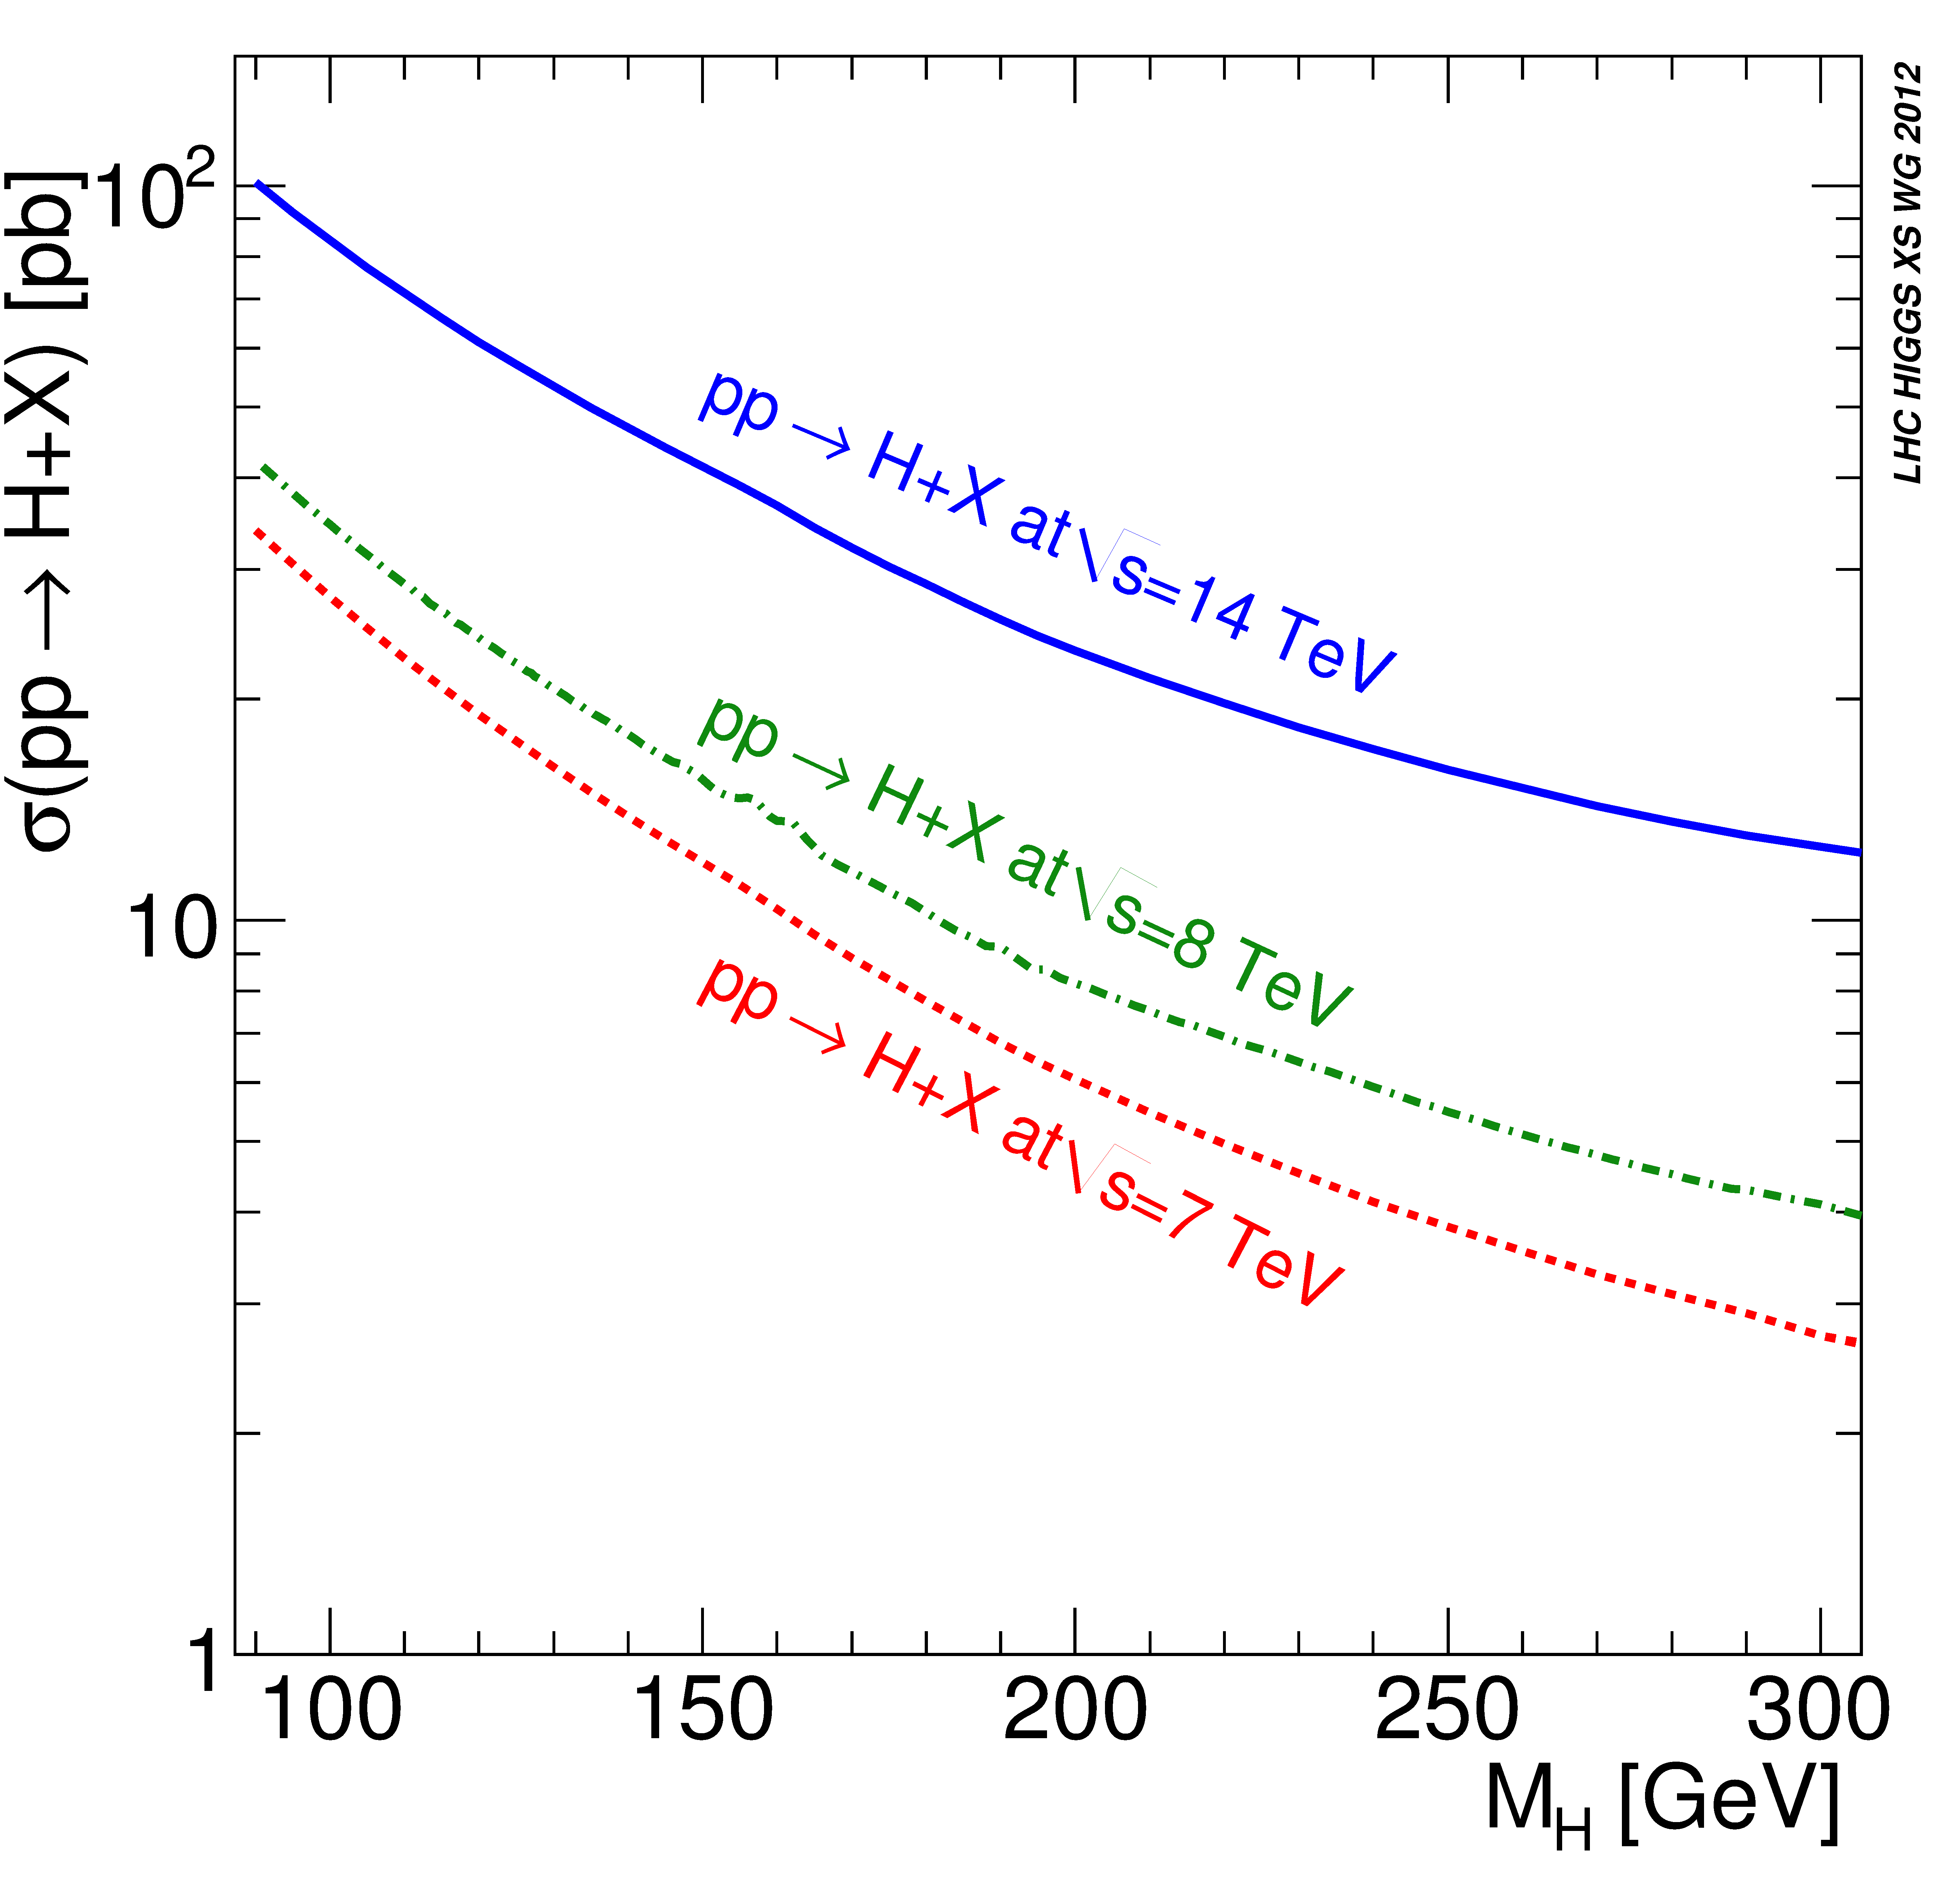
\includegraphics[width=0.8\textwidth]{../figs/totalXS_LM.png}
  \end{center}
\end{figure}

\end{column}
\end{columns}

\end{frame}

\fi